\centering
\begin{blackbox}{Textual Representation}
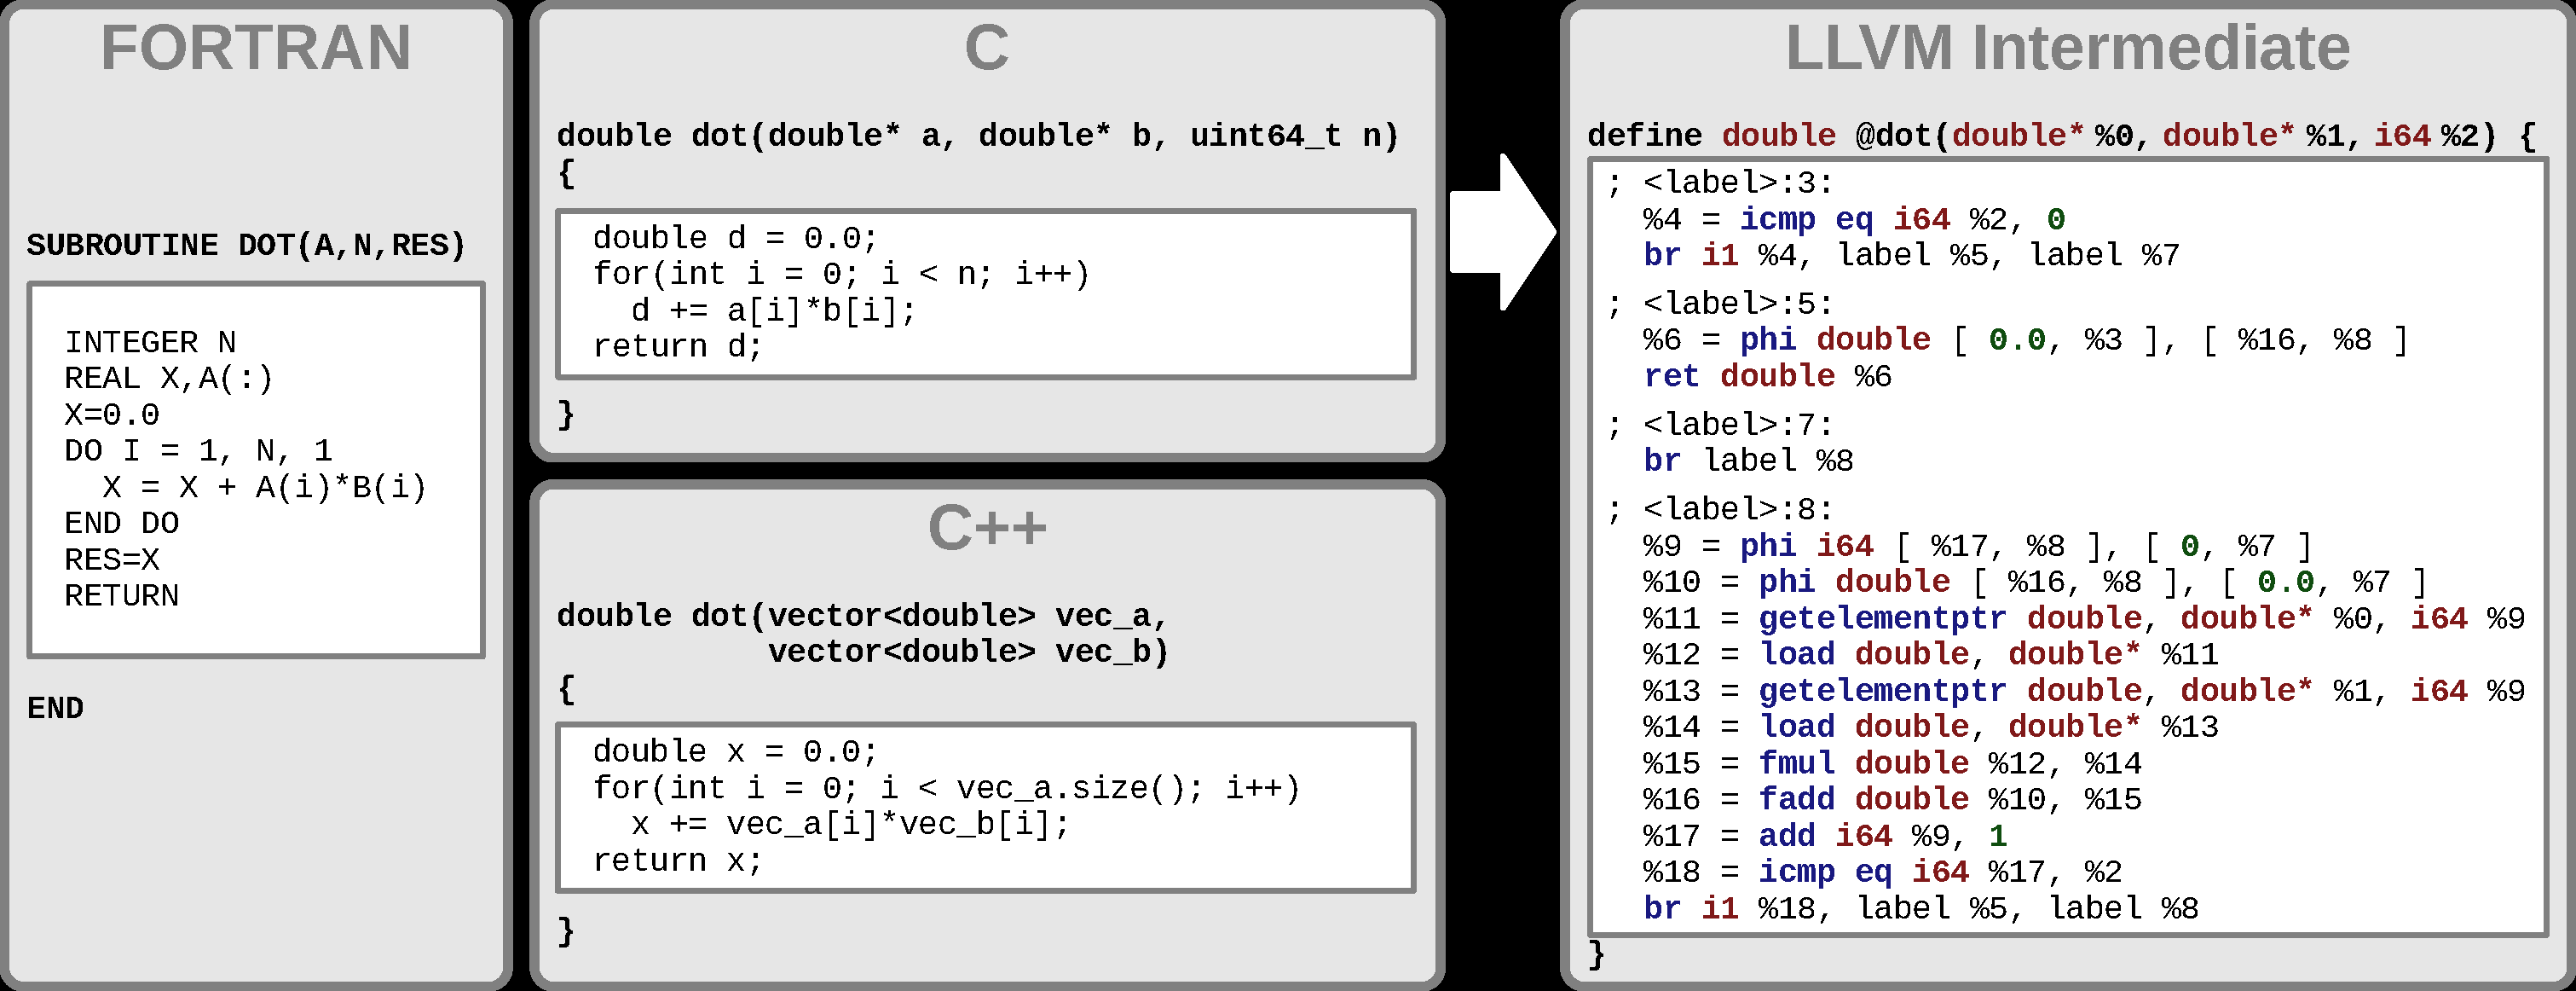
\includegraphics[width=\columnwidth]{figures/model_representations_textual}
\end{blackbox}


\includegraphics[width=\columnwidth]{figures/model_arrows_upper}

\begin{blackbox}{Data Structure Representation}
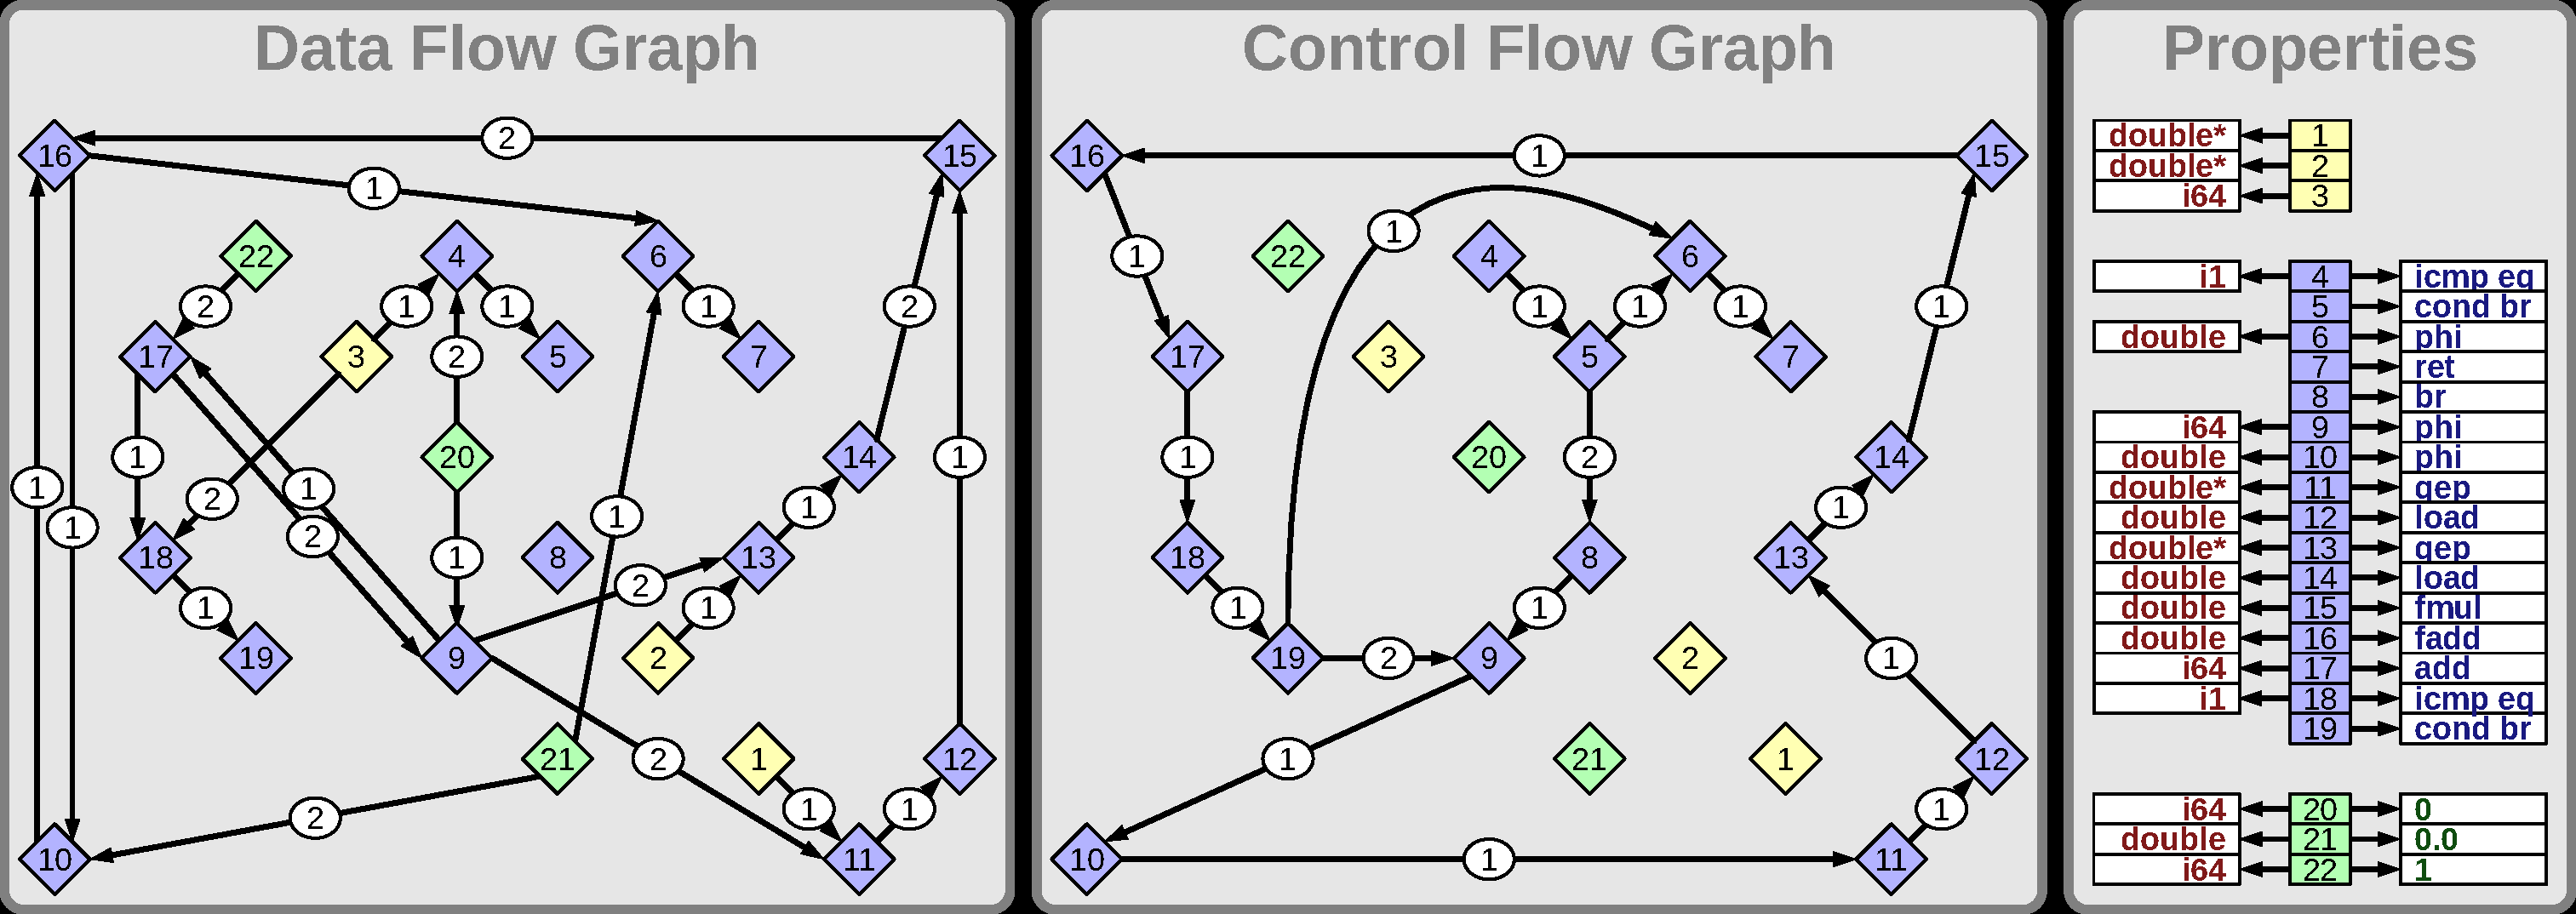
\includegraphics[width=\columnwidth]{figures/model_representations_structure}
\end{blackbox}

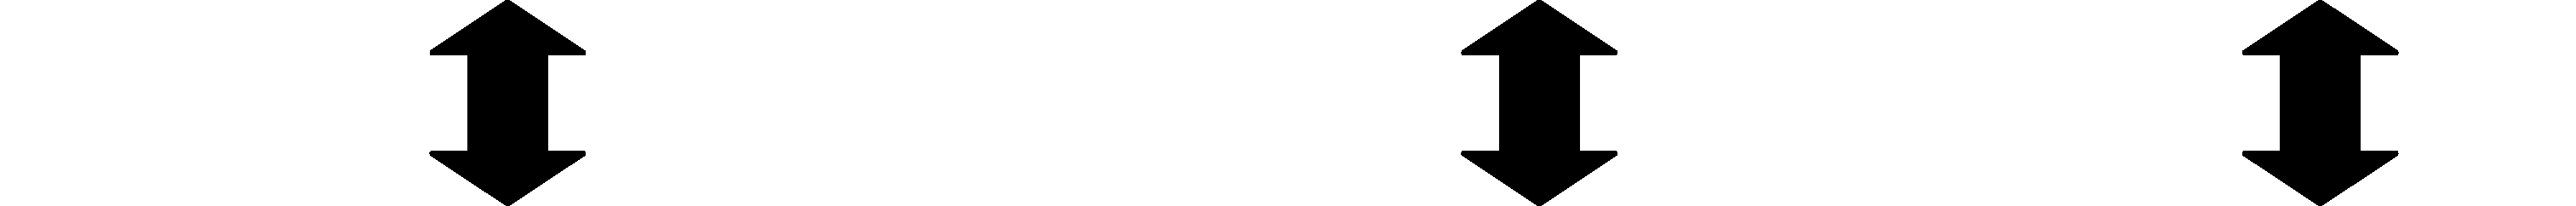
\includegraphics[width=\columnwidth]{figures/model_arrows_lower}

\begin{blackbox}{Mathematical Representation}
    \centering
    \begin{minipage}{0.329\textwidth}
        \begin{graybox}
            \scriptsize
            \setlength{\abovedisplayskip}{0pt}
            \setlength{\belowdisplayskip}{0pt}
            \vspace{-0.5em}
            \begin{align*}
                DF&G_\mathcal F=\{(1,11,1),(2,13,1)\\[-0.5em]
                  &(3,4,1),(3,18,2),(4,5,1),\\[-0.5em]
                  &(6,7,1),(9,11,2),(9,13,2),\\[-0.5em]
                  &(9,17,1),(10,16,1),(11,12,1),\\[-0.5em]
                  &(12,15,1),(13,14,1),(14,15,2),\\[-0.5em]
                  &(15,16,2),(16,6,1),(16,10,1),\\[-0.5em]
                  &(17,9,2),(17,18,1),(18,19,1),\\[-0.5em]
                  &(20,4,2),(20,9,1),(21,6,1),\\[-0.5em]
                  &(21,10,2),(22,17,2)\}\subset\mathbb N^3
            \end{align*}
        \end{graybox}
    \end{minipage}
    \begin{minipage}{0.329\textwidth}
        \begin{graybox}
            \scriptsize
            \setlength{\abovedisplayskip}{0pt}
            \setlength{\belowdisplayskip}{0pt}
            \vspace{-0.5em}
            \begin{align*}
                CFG_\mathcal F=\{&(4,5,1),(5,6,1),\\[-0.5em]
                  &(5,8,2),(6,7,1),\\[-0.5em]
                  &(8,9,1),(9,10,1),\\[-0.5em]
                  &(10,11,1),(11,12,1),\\[-0.5em]
                  &(12,13,1),(13,14,1),\\[-0.5em]
                  &(14,15,1),(15,16,1),\\[-0.5em]
                  &(16,17,1),(17,18,1),\\[-0.5em]
                  &(18,19,1),(19,6,1),\\[-0.5em]
                  &(19,9,2)\}\subset\mathbb N^3
            \end{align*}
        \end{graybox}
    \end{minipage}
    \begin{minipage}{0.329\textwidth}
        \centering
        \begin{graybox}
            \scriptsize
            \setlength{\abovedisplayskip}{0pt}
            \setlength{\belowdisplayskip}{0pt}
            \vspace{-0.5em}
            \begin{align*}
                T_\mathcal F={}&\{(1,\textit{double*}),(2,\textit{double*}),\dots\}\\[-0.5em]
                      \subset{}&\mathbb N\times Types_\text{LLVM}\\[-0.25em]
                P_\mathcal F={}&\{1,2,3\}\subset\mathbb N\\[-0.25em]
                I_\mathcal F={}&\{(4,\textit{icmp eq}),(5,\textit{cond br}),\dots\}\\[-0.5em]
                      \subset{}&\mathbb N\times Opcodes_\text{LLVM}\\[-0.25em]
                G_\mathcal F={}&\{\}\subset\mathbb N\\[-0.25em]
                C_\mathcal F={}&\{(20,0),(21,0),(22,1)\}\\[-0.5em]
                      \subset{}&\mathbb N\times\mathbb R
            \end{align*}

            \vspace{0.45em}
        \end{graybox}
    \end{minipage}

    \begin{minipage}{0.55\textwidth}
        \begin{graybox}
            \setlength{\abovedisplayskip}{0pt}
            \setlength{\belowdisplayskip}{0pt}
            \vspace{-0.5em}
            \begin{align*}
                M_{dot}=(DFG_\mathcal{F},
                 CFG_\mathcal{F},
                 T_\mathcal{F},
                 P_\mathcal{F},
                 I_\mathcal{F},
                 G_\mathcal{F},
                 C_\mathcal{F})
            \end{align*}
        \end{graybox}
    \end{minipage}
\end{blackbox}